\section{Dokumentáció}\label{sec:dokumentacio}

\subsection{Logikai adatfolyam-diagramok}

\begin{figure}[!htb]

    \centering
    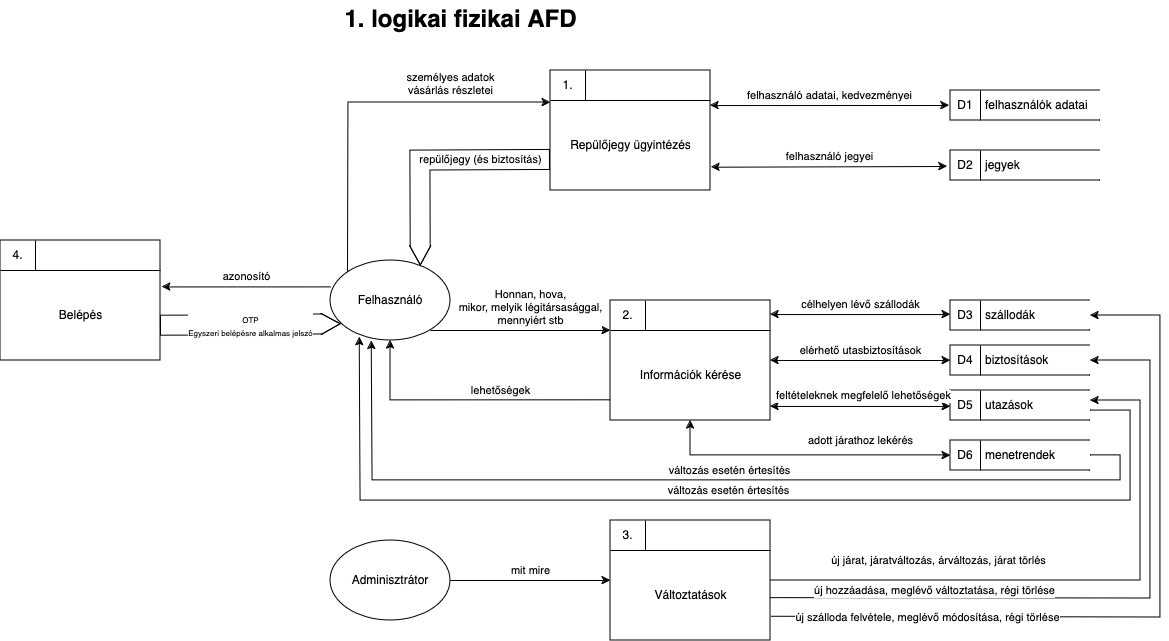
\includegraphics[scale=0.37]{logical1}
    \caption{\label{fig:logical1}Logikai AFD 1. szinten}

\end{figure}

\begin{figure}[!htb]

    \centering
    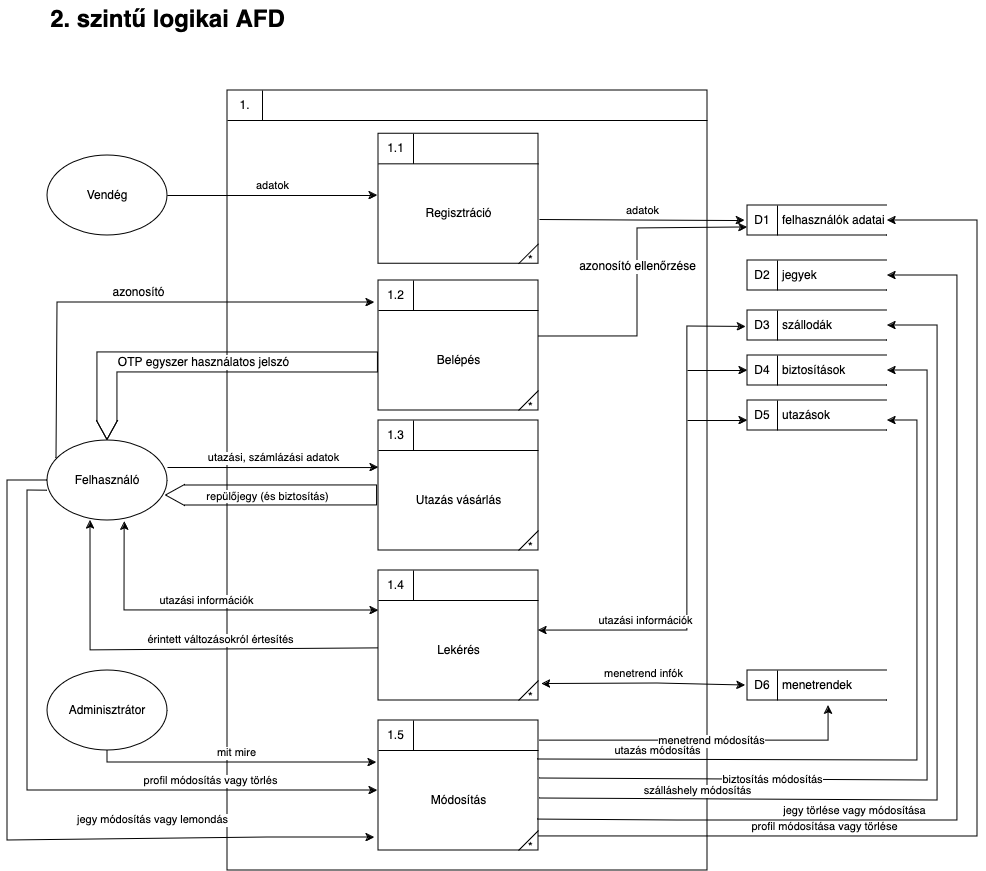
\includegraphics[scale=0.37]{logical2}
    \caption{\label{fig:logical2}Logikai AFD 2. szinten}

\end{figure}
\pagebreak

\subsection{Fizikai adatfolyam-diagramok}

\begin{figure}[!htb]

    \centering
    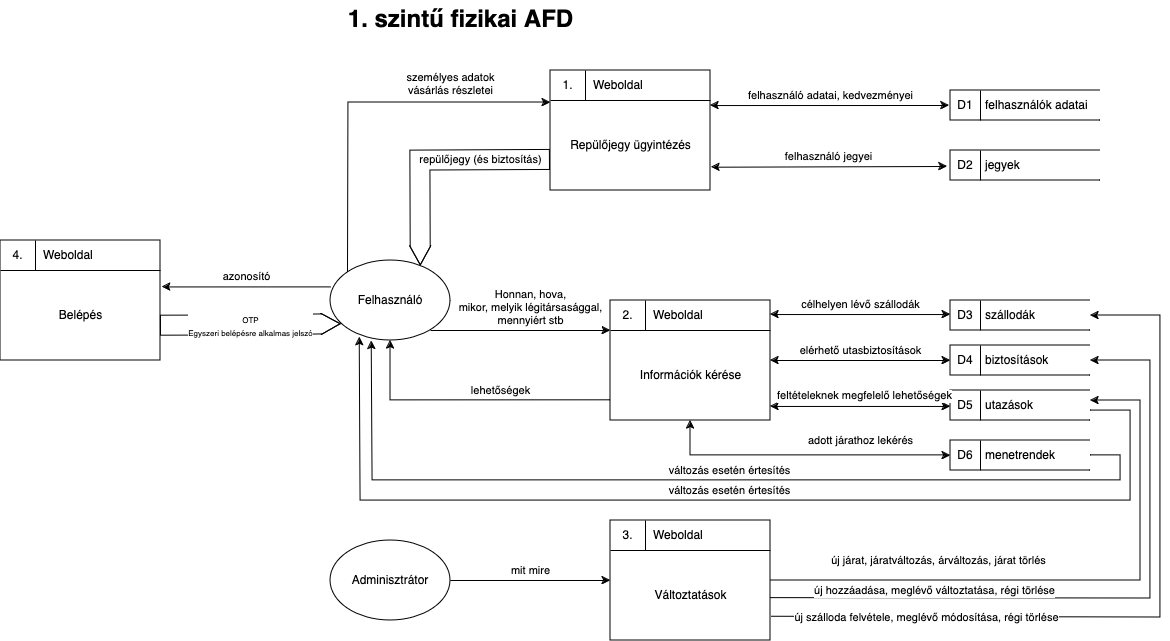
\includegraphics[scale=0.37]{physical1}
    \caption{\label{fig:physical1}Fizikai AFD 1. szinten}

\end{figure}

\begin{figure}[!htb]

    \centering
    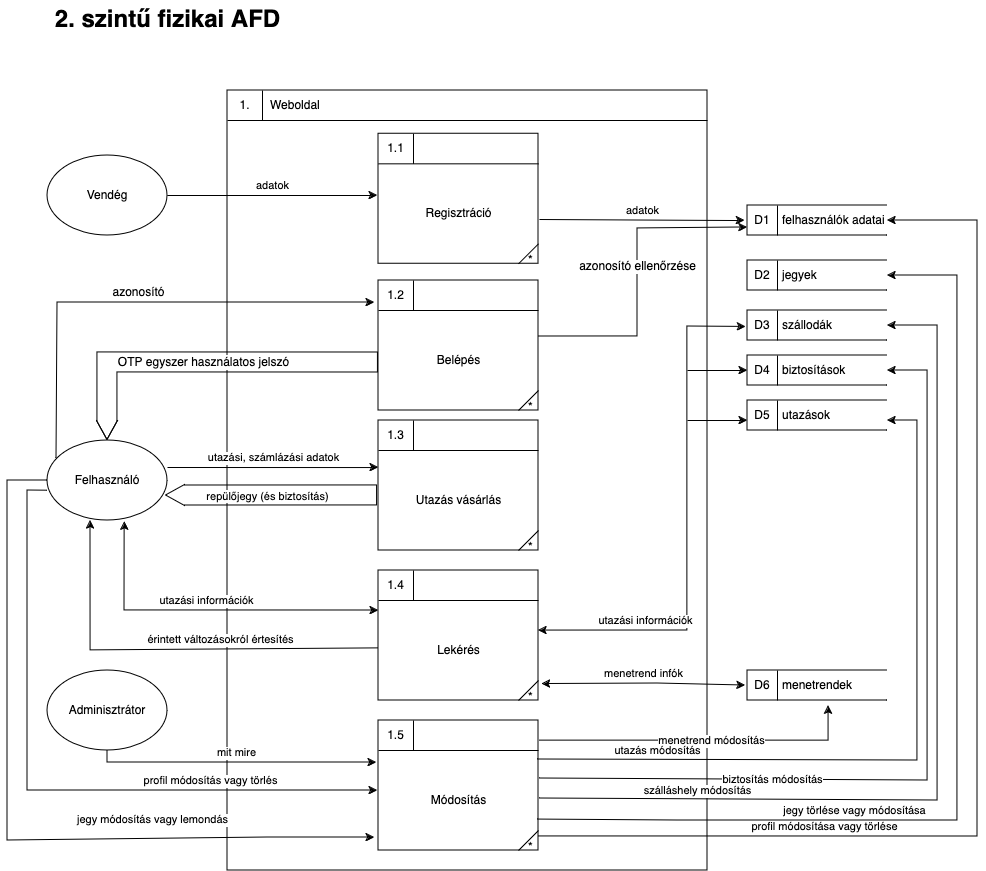
\includegraphics[scale=0.37]{physical2}
    \caption{\label{fig:physical2}Fizikai AFD 2. szinten}

\end{figure}
\pagebreak

\subsection{Egyedmodell}

\begin{figure}[!htb]

    \centering
    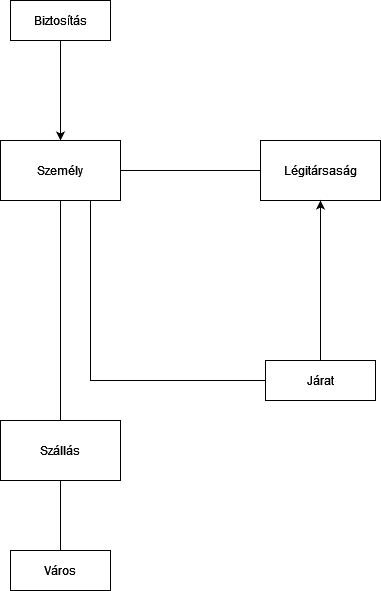
\includegraphics[scale=0.37]{egyedkapcsolat_diagram}
    \caption{\label{fig:egyedkapcsolat_diagram}Fizikai AFD 2. szinten}

\end{figure}
\pagebreak

\subsection{E-K Diagram}

\begin{figure}[!htb]

    \centering
    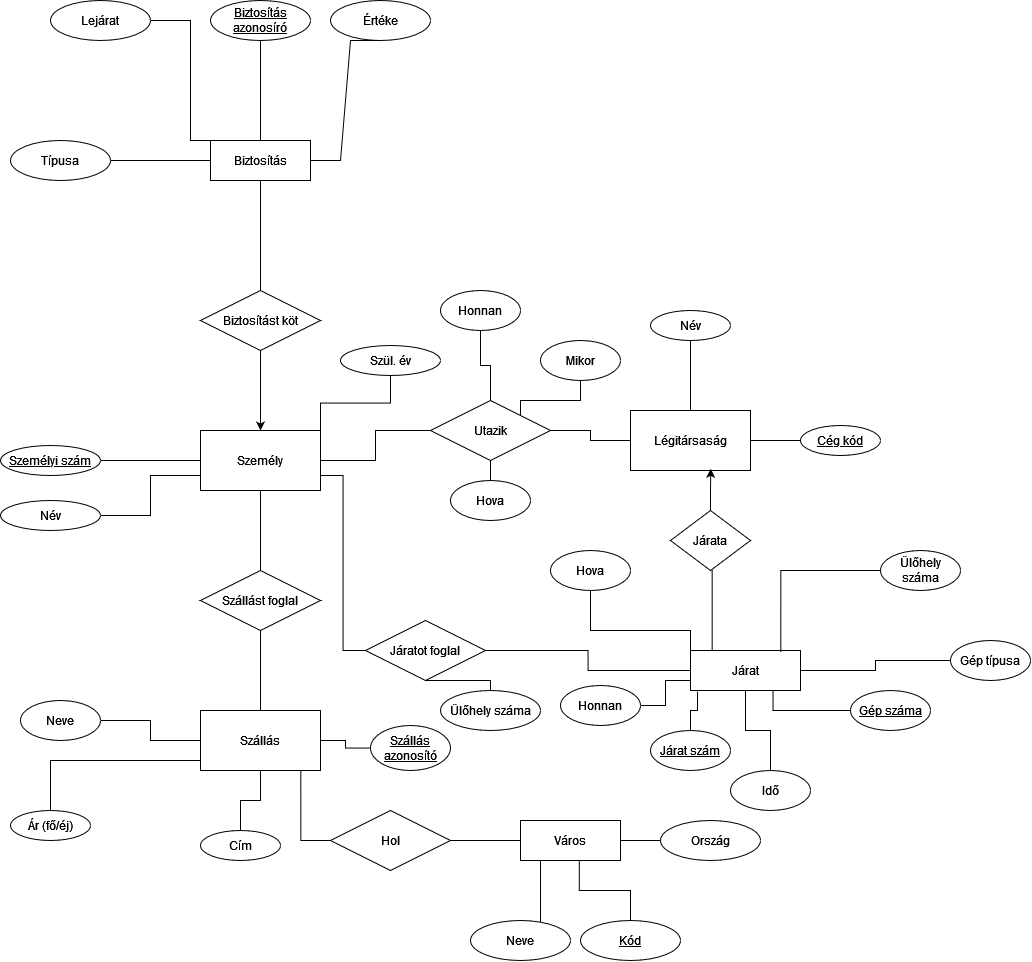
\includegraphics[scale=0.40]{e-k_diagram}
    \caption{\label{fig:e-k_diagram}E-K Diagram}

\end{figure}
\pagebreak
\subsection{Egyed-kapcsolat diagram leképezése relációs sémákká}

    BIZTOSÍTÁS(\underline{Biztosítás azonosító},Típus, Lejárat, Értéke)\\
    SZEMÉLY(\underline{Személyi szám}, Név, Szül. év)\\
    SZÁLLÁS(\underline{Szállás azonosító}, Neve, Ár (fő/éj), Cím)\\
    VÁROS(\underline{Kód} ,Neve, Ország)\\
    LÉGITÁRSASÁG(\underline{Cég kód}, Név)\\
    JÁRAT(\underline{Járat szám},\underline{Gép száma}, Hova, Honnan, Idő, Gép típusa, Ülőhely száma)
